\begin{blocksection}
\question Give the environment diagram and console output that result from running the following code.

\begin{lstlisting}
x = 20
def foo(y):
    x = 5
    def bar():
        return lambda y: x - y
    return bar

y = foo(7)
z = y()
print(z(2))
\end{lstlisting}

\begin{solution}[2in]
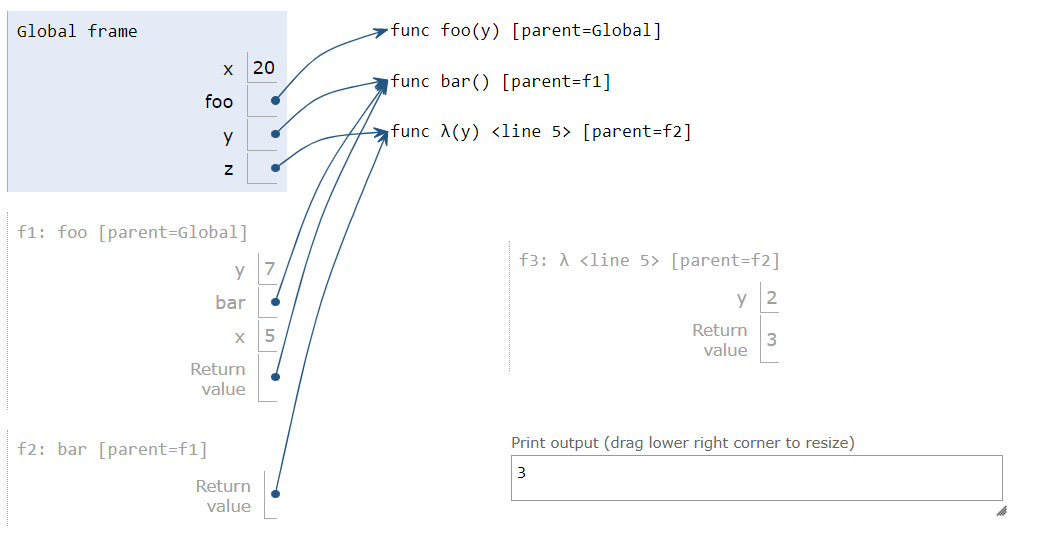
\includegraphics[scale=0.5]{foobar.png}
\\
\url{https://tinyurl.com/yxfcvxxa}
\end{solution}
\end{blocksection}

\begin{guide}
    \begin{blocksection}
    \textbf{Teaching Tips}
      \begin{itemize}
        \item Make sure that your students understand the process of looking up a value of a variable in Python
      \end{itemize}
    \end{blocksection}
\end{guide}
    